% TODO - WORK IN PROGRESS
\section{Covert Channel on IoT Light Bulb} % ~ 1/4 page (short intro)
\label{sec:experiment}
Our goal was to reproduce the attack from Ronen \& Shamir~\cite{Ronen:2016:EFAIDCSL}.
Therefore, we tried building a covert channel using the \textit{Philips Hue White} lighting system. With our experiment we were able to prove that data can be covertly transmitted using the Hue light bulb. 
On the transmission side we used a laptop running our python script over which the Hue API is accessed in order to send brightness commands.
At the receiver side we used a light sensor which converts the light intensities to a frequency signal. That signal was forwarded to an oscilloscope which further sent the received frequency output to our laptop where we plot the results in order to validate the sent bits.

In the following sections we first describe the setup components and their functionality. After that, we elaborate the actual attack.\newline

\subsection{Experimental Setup} % ~ 2 pages (including subsections bulb to pico)
\label{sec:setup}

% picoscope ~1000 €
% light sensor ~7 €
% bulbs ~70 €
% arduino etc ~10-20 €
% --> overall: less than 1100 €

Our proof of concept was implemented using affordable equipment which costs less than 1100.- €. Further, we did not need to run any unauthorized code on the light bulbs since the control over the Hue API suffices to create covert flicker effects. 
Figure \ref{fig:setup} shows our overall receiving setup. An Arduino was used as power supply and for configuring the light sensor, which the Picoscope had direct access to.
\begin{figure}[h]
	\centering
	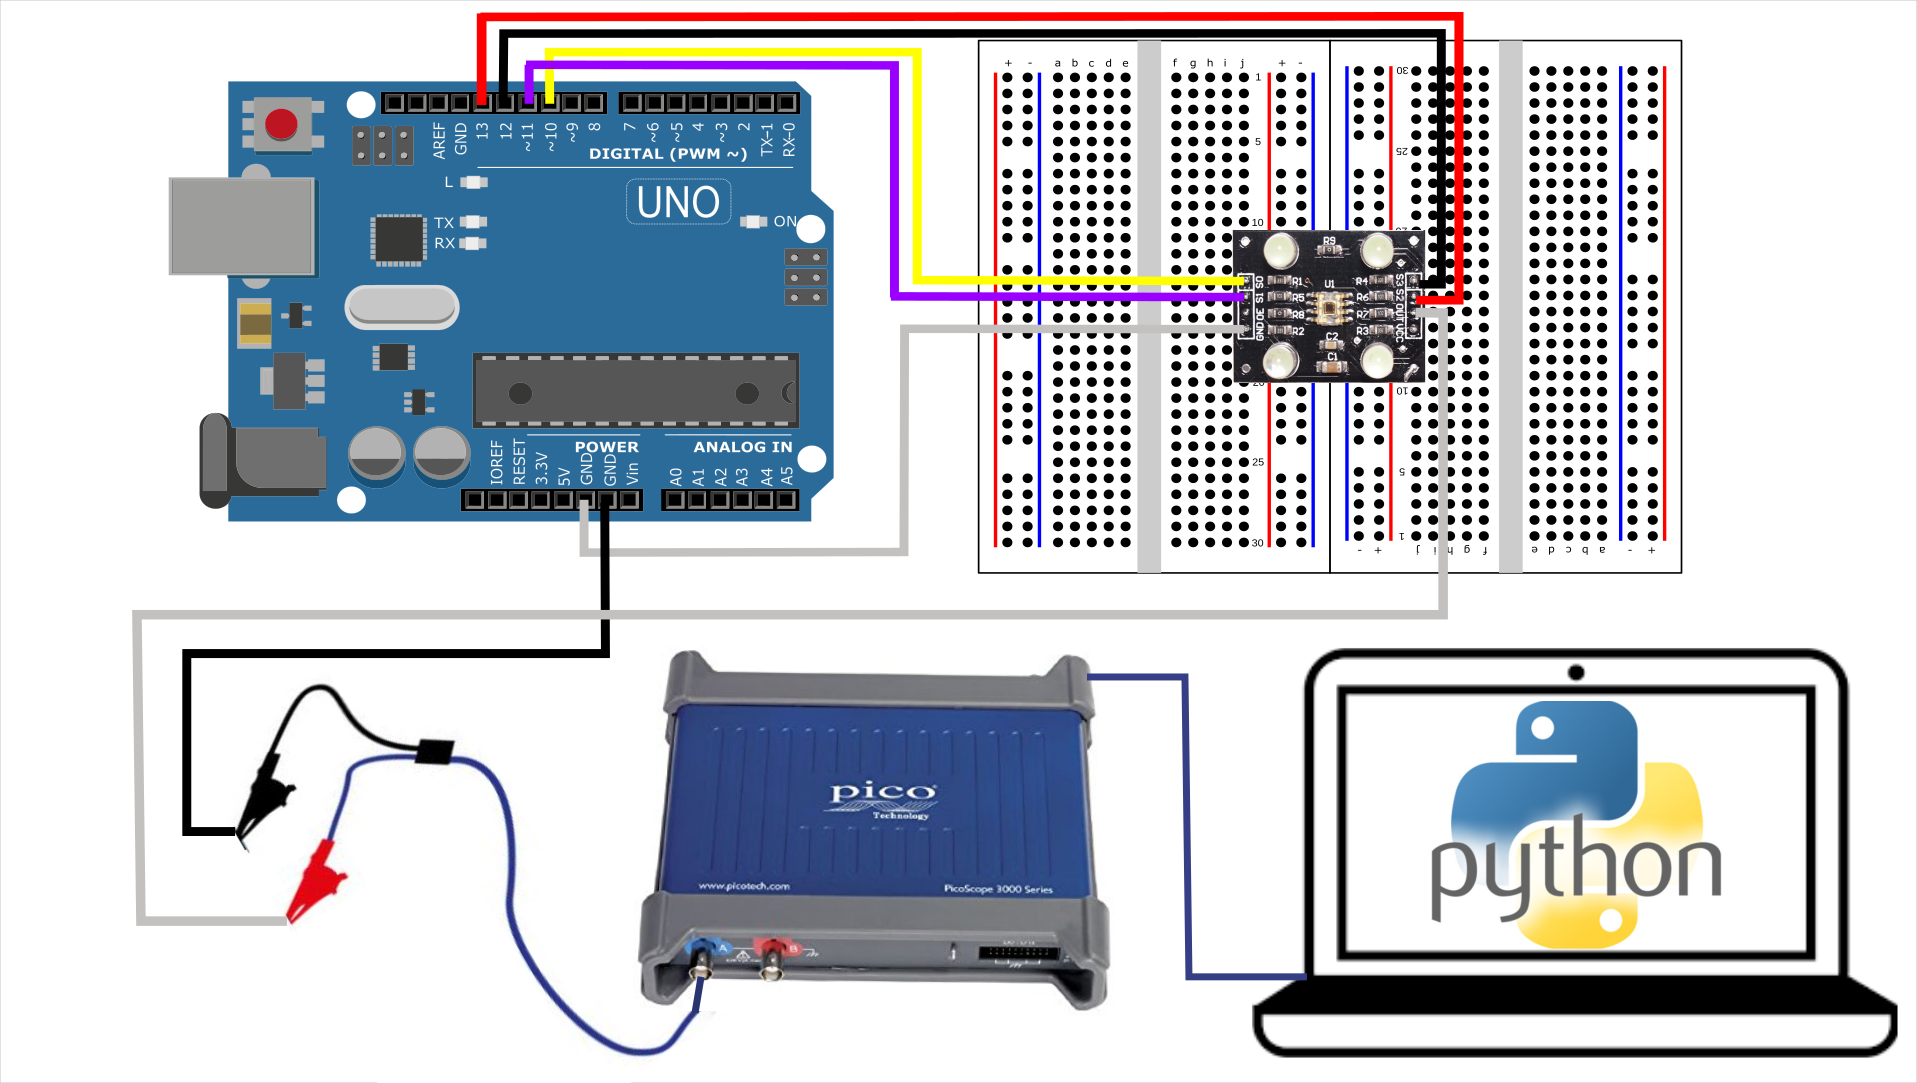
\includegraphics[width=14cm]{img/experimental-setup_overview.png}
	\caption{Experimental setup for measuring the lights frequency output and reading the sent bits out of the received signal}
	\label{fig:setup}
\end{figure}

\subsubsection{Transmitting Setup.} We used the \textit{Philips~Hue~White} light bulbs for our experiment~\cite{Philips:2018:Hue}. We bought the starter kit which contains two E27 9 Watt 806 Lumen bulbs together with a bridge which allows to remotely control the bulbs using i.~e. a laptop. In order to set up the smart light system the bridge needs to be connected to the user's network using Ethernet. Once connected, the user can send brightness-change commands from any device within the local network using the Hue~API. We made recourse to a command line based version of the Hue~API~\cite{Bahamas10:2018:HueApi}, which allowed us to easily send the commands via the python script we used for realizing the experiment. The bridge further forwards the commands over a radio frequency (RF) transmitter to the light bulbs using the ZLL protocol.

The Hue White bulbs have 255 different brightness levels, which forced us to sample the output at a very hight rate in order to determine the changes in the light frequency output. But, on the other hand, due to the minor difference between two close levels, the changes were imperceptible to the human eye, which worked for us.

\subsubsection{Receiving Setup.} For measuring the changes in light intensity we used the \textit{TAOS~TCS3200 Color~Sensor}~\cite{DFRobot:2018:Sensor}. The sensor consists of an array of photo diodes where each is capable of filtering red, green, blue or clear white light. We set up the sensor to measure the clear white luminosity output of our Hue bulbs. The sensor contains an internal oscillator in order to convert the light's intensity output to a corresponding square-wave frequency signal. The TCS3200 is capable of communicating directly to an Arduino microcontroller.

Unlike Ronen and Shamir~\cite{Ronen:2016:EFAIDCSL}, we used the Arduino board as power source only, and the Picoscope to measure the brightness. This was necessary because the advanced API functionality which the former used to craft a PWM signal is no longer available~\cite{Ronen:2016:EFAIDCSL}, and we had to directly distinguish existing brightness levels using their PWM profile.

In order capture the output from the light sensor, we used the \textit{PicoScope~3205D~MSO} since it is capable of sampling 10~MS/s, which we need in order to accurately measure the light sensor's frequency output which lies around 800 KHz. Actually, the picoscope is able to sample up to 1~GS/s when using one channel and 500 MS/s with two channels, but for our needs only 10~MS/s suffice.

